\documentclass[a4paper, 12pt]{article}
\usepackage[utf8]{inputenc}
\renewcommand\familydefault{\sfdefault}
\usepackage[T1]{fontenc}
\usepackage[francais]{babel}
\usepackage[left=2.4cm,top=2.4cm,right=2.4cm,bottom=2.4cm]{geometry}
\usepackage{graphicx}
\usepackage{minted}
\usemintedstyle{colorful}
\usepackage{float}
\floatplacement{figure}{H}
\usepackage{authblk}
\usepackage{enumitem}
\usepackage{hyperref} 
\hypersetup{
	colorlinks,
	citecolor=black,
	filecolor=black,
	linkcolor=black,
	urlcolor=blue
}

\usepackage{caption}
\newenvironment{code}{\captionsetup{type=listing}}{}

\begin{document}

\title{Petits comptes entre amis} 
\author{Steven Liatti} 
\affil{\small Développement et services web - Prof. Stéphane Malandain} 
\affil{\small Hepia ITI 3\up{ème} année} 
\maketitle

\begin{figure}
	\begin{center}
		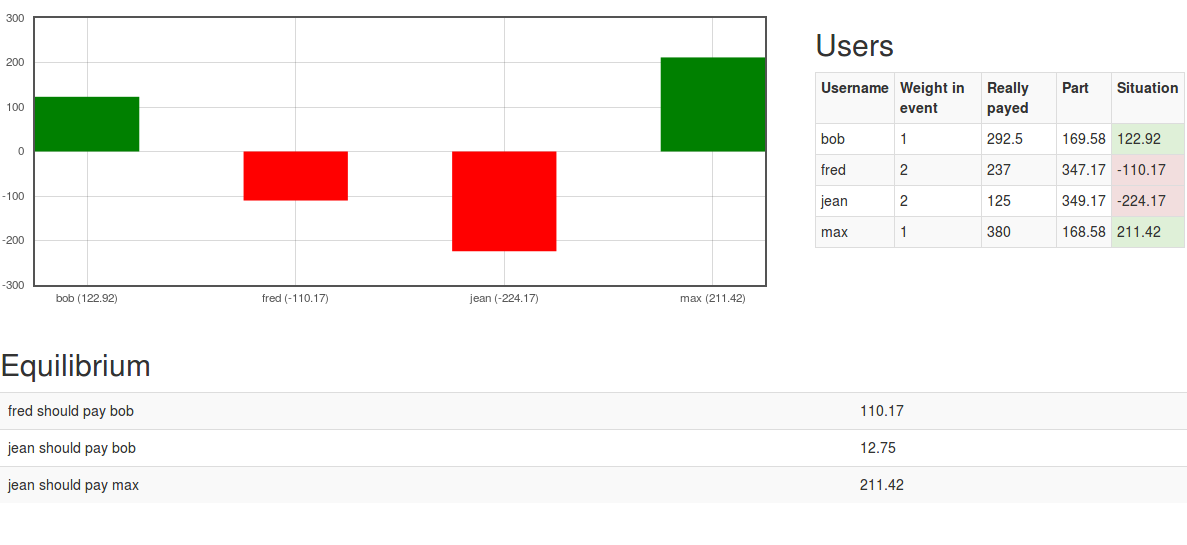
\includegraphics[width=1.0\textwidth]{intro.png}
	\end{center}
\end{figure}
\newpage

\tableofcontents
\listoffigures
\renewcommand\listoflistingscaption{Table des listings de code source}
\listoflistings

\newpage

\section{Introduction}
\subsection{Description}
Le but de ce mini-projet est de réaliser un site en PHP permettant à des amis de noter et
partager les dépenses effectuées par et pour le groupe au cours de vacances
communes. Lorsque l'une des personnes fait des courses, par exemple, elle l'enregistre.
Chacun enregistre les dépenses qui concernent le groupe. Ainsi, à la fin du séjour (ou à
tout moment) on peut savoir qui a payé quoi et surtout ce que chacun doit aux autres
personnes du groupe d'amis.

\subsection{Technologies utilisées}
\begin{itemize}
	\item Base de données :
	\begin{itemize}
		\item \href{https://www.mysql.com/}{MySQL}, avec
		\item \href{https://www.mysql.com/products/workbench/}{MySQL Workbench} (pour la création du schéma)
	\end{itemize}
	\item Back-end :
	\begin{itemize}
		\item \href{https://httpd.apache.org/}{Apache}, serveur HTTP
		\item \href{http://php.net/}{PHP}, avec
		\item \href{https://silex.symfony.com/}{Silex}, micro framework PHP basé entre autres sur \href{https://symfony.com/}{Symfony}, déployé avec \href{https://getcomposer.org/}{Composer}
		\item \href{https://twig.symfony.com/}{Twig}, moteur de templates pour PHP (utilisé de concert avec Silex)
	\end{itemize}
	\item Front-end :
	\begin{itemize}
		\item \href{http://getbootstrap.com/}{Bootstrap} pour le design en CSS
		\item \href{https://jquery.org/}{jQuery}
		\item \href{http://www.flotcharts.org/}{Flot}, un plugin pour dessiner des graphiques avec jQuery
	\end{itemize}
\end{itemize}

\subsection{Déploiement du site}
Les fichiers du site sonts disponibles ici : \url{https://github.com/steenput/web_pcea}
Pour déployer le site, il faut commencer par avoir Apache, PHP et MySQL installés. Pour créer la base de données 
et les tables il suffit d'exécuter \mintinline{text}{db/schema.sql} dans MySQL. Du contenu pour tester est 
présent dans \mintinline{text}{db/content.sql}. Il est également nécessaire d'adapter la configuration dans 
\mintinline{text}{app/config/prod.php}. Il faut ensuite, dans un terminal, se déplacer à la racine du site 
(dans le dossier Apache ou autres) et, avec Composer installé, exécuter \mintinline{shell}{composer install}. 
Toutes les dépendances du projet vont automatiquement s'ajouter dans le dossier \mintinline{text}{vendor}.
Il faut donner les bons droits au fichier \mintinline{text}{var/logs/pcea.log} pour que le composant de 
logs (Monolog) puisse y écrirer dedans. À noter que les droits administrateurs seront sûrement demandés. 
Enfin, il est nécessaire d'avoir une connexion à internet (Bootstrap et jQuery sont appelés grâce à des CDN).

\section{Base de données}
Les technologies imposées pour la base de données de ce travail pratique sont SQLite ou MySQL. J'ai choisi 
d'utiliser MySQL, car je suis familier avec. J'ai profité de cette occasion pour découvrir et utiliser Workbench, 
un programme permettant de modéliser les tables et relations d'une base de données de manière graphique. Une fois 
le model terminé, Workbench offre la possibilité de l'exporter en instructions SQL (création de tables et 
contraintes).
\bigbreak

Mon schéma est constitué des tables suivantes :
\begin{figure}
	\begin{center}
		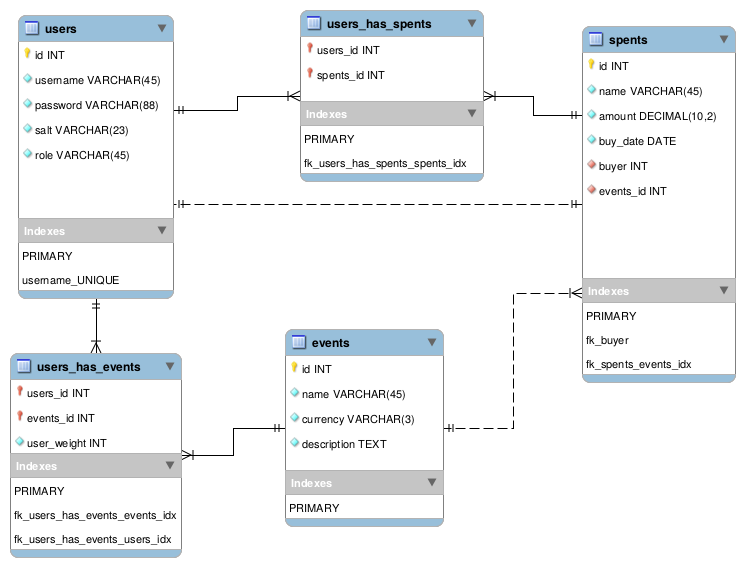
\includegraphics[width=1.0\textwidth]{database.png}
	\end{center}
	\caption{Schéma de la base de données relationnelle}
\end{figure}
Il y a 3 tables principales : les utilisateurs, les événements et les dépenses. 2 autres tables secondaires 
font la liaison entre les utilisateurs et les événements et les utilisateurs et les dépenses respectivement 
(liaison Many-To-Many). La table des utilisateurs possède un champ \mintinline{sql}{salt} et un autre 
\mintinline{sql}{role}, ils sont nécessaires au fonctionnement de Silex (voir listing \ref{controller_register}). 
Le poids de chaque utilisateur au sein d'un événement est indiqué dans la table croisée 
\mintinline{sql}{users_has_events}. 
Chaque dépense référence l'acheteur (dans \mintinline{sql}{users}) et l'événement lié (dans \mintinline{sql}
{events}). Ce schéma représente l'interface minimum pour les données de ce travail, mais il a l'avantage 
d'être simple à comprendre et à maintenir.

\section{Back-end}
Je profite également de ce TP pour appréhender Silex, un micro framework PHP dérivé de Symfony (que j'ai eu 
l'occasion de tester), beaucoup plus léger que son grand frère mais tout de même robuste et modulaire. Il 
bénéficie d'un grand nombre de modules à ajouter, en vrac : système de templates, connexion à la base de données, 
routes, etc.

\newpage

\subsection{Architecture MVC avec Silex}
Grâce à Silex, mon architecture respecte le design pattern \href{https://en.wikipedia.org/wiki/Model-view-controller}{MVC}.
On peut configurer Silex pour que le code source, défini dans le répertoire \mintinline{text}{src}, soit ajouté 
au mécanisme de chargement automatique (autoloading) géré par Composer. Pour que cela fonctionne, il faut que le code 
source respecte le standard \href{http://www.php-fig.org/psr/psr-4/}{PSR-4}.
Voici l'arborescence du site :
\begin{code}
	\inputminted[breaklines,breaksymbol=,linenos,frame=single,stepnumber=5,tabsize=2]{text}{tree.txt}
	\caption{Arborescence du site}
	\label{tree}
\end{code}
\newpage
\begin{itemize}
	\item app : fichiers de config et routes
	\item composer.json : fichier de dépendances
	\item src : fichiers source PHP ("POPO", DAO, Contrôleurs)
	\item var : logs
	\item vendor : fichiers sources des composants Silex/Symfony
	\item views : fichiers de vues en Twig
	\item web : fichiers CSS, JS, images, etc. publics livrés au client
\end{itemize}

\subsection{Composants Silex}
Silex fournit plusieurs composants vraiment pratiques et très efficaces. Les composants suivants m'ont été 
particulièrement utiles :
\begin{itemize}
	\item Un composant de sécurité qui gère le login des utilisateurs
	\item Un composant de construction de formulaires
	\item Un composant pour se connecter à la base de données
	\item Un composant de rendu de templates (Twig)
	\item Un composant permettant de facilement appliquer des contraintes pour valider les données
\end{itemize}

\subsection{Routage et configuration}
Dans le dossier \mintinline{text}{app} se trouvent les fichiers de configuration (pour MySQL notamment) et les 
déclarations/configurations des modules et composants récupérés grâce à Composer (dans \mintinline{php}{app/app.php}).
Le point d'entrée du site est \mintinline{text}{web/index.php}. C'est le contrôleur frontal, c'est par ici que 
toutes les requêtes passent (grâce au fichier de configuration d'Apache \mintinline{text}{.htaccess}). 
Il instancie l'objet principal \mintinline{php}{$app} et fait suivre aux fichier de routes. Silex permet de 
définir des routes, c'est-à-dire des points d'entrée dans l'application. À chaque route est associée une action 
(requête GET et/ou POST) définie dans un contrôleur. Pour ce site, j'ai défini 6 routes : page d'accueil (avec 
formulaires de connexion et d'inscription), page d'un événement, nouvel événement, nouvelle dépense, suppression 
d'événement et suppression de dépense.

\subsection{Modèles, accès aux données}
\label{data_model_access}
L'accès aux données avec Silex/Symfony se fait généralement avec l'ORM 
\href{http://docs.doctrine-project.org/en/latest/}{Doctrine} (l'utilisation de base est semblable à PDO PHP) 
selon le modèle Data Access Object (DAO). 
Tout ce qui touche cet accès se trouve dans les classes \mintinline{php}{src/DAO/xxxDAO.php}, avec pour chaque 
fichier les requêtes traitant avec la table du même nom. La classe \mintinline{php}{src/DAO/UserDAO.php} a une 
contrainte supplémentaire, elle implémente l'interface \mintinline{php}{UserProviderInterface} nécessaire au 
fonctionnement du module de sécurité/login des utilisateurs. Pour les besoins de la construction des formulaires, 
des vues et pour un code plus modulaire, chaque table est représentée par un 
"\href{https://en.wikipedia.org/wiki/Plain_old_Java_object}{POPO}", un simple objet PHP avec attributs et 
accesseurs. Voici par exemple l'insertion d'un nouvel événement en base de données (voir listing 
\ref{insert_event}) :
\newpage
\begin{code}
	\inputminted[breaklines,breaksymbol=,linenos,frame=single,stepnumber=5,tabsize=2,firstline=36,lastline=58]{php}{../src/DAO/EventDAO.php}
	\caption{Insertion d'un événement - \mintinline{php}{src/DAO/EventDAO.php}}
	\label{insert_event}
\end{code}

\subsection{Contrôleurs}
Les contrôleurs sont le socle de ce site, c'est ici que sont récupérées les requêtes et les données (grâce aux 
DAO) et construits les formulaires et les vues. Une fonction \mintinline{php}{xxxAction()} d'un contrôleur a 
pratiquement toujours la forme suivante : test si la page est accessible par le client qui la demande, 
récupération des données (voir la sous-section \ref{data_model_access}), si besoin 
construction/vérification/validation des formulaires et enfin rendu de la vue ou redirection vers une page donnée.

\subsubsection{\mintinline{php}{IndexController.php}}
Ce contrôleur gère les actions de la page principale. Si un utilisateur est connecté, il lui affiche les 
événements auxquels ils participe. Sinon, deux formulaires, de login et d'inscription, sont affichés. Grâce au 
composant de sécurité intégré, j'ai facilement pu mettre en place le login utilisateur. Il m'a suffit de 
configurer quelques réglages dans \mintinline{php}{app/app.php} : la route du formulaire de login et celle de la 
vérification du login (automatiquement faite), si les clients anonymes peuvent accéder à la page principale, 
la provenance des données utilisateurs, etc. (voir listing \ref{config_login}) :
\begin{code}
	\inputminted[breaklines,breaksymbol=,linenos,frame=single,stepnumber=5,tabsize=2,firstline=26,lastline=39]{php}{../app/app.php}
	\caption{Configuration du login utilisateur - \mintinline{php}{app/app.php}}
	\label{config_login}
\end{code}
\bigbreak

Si l'utilisateur s'inscrit, 
son formulaire est construit grâce au composant Silex dédié, et lorsqu'il est reçu valide et conforme en retour, 
son mot de passe est chiffré avec bcrypt et le nouvel utilisateur est inscrit en base de données (voir listing 
\ref{controller_register}) :
\begin{code}
	\inputminted[breaklines,breaksymbol=,linenos,frame=single,stepnumber=5,tabsize=2,firstline=22,lastline=56]{php}{../src/Controller/IndexController.php}
	\caption{Inscription d'un utilisateur - \mintinline{php}{src/Controller/IndexController.php}}
	\label{controller_register}
\end{code}

\subsubsection{\mintinline{php}{EventController.php}}
Ce contrôleur gère les actions des pages des événements et des dépenses. Les actions de créer et supprimer 
dépenses et événements sont semblables, le formulaire est créé, envoyé au client, au retour il est vérifié 
et si tout est en ordre on enregistre la nouvelle entrée en base de données. L'action d'afficher l'événement 
avec ses dépenses et l'équilibre est un peu plus longue. Je commence par effectuer un tableau des parts de 
chaque membre puis je calcule la situation pour chacun (positive ou négative) et finalement, en parcourant 
plusieurs fois le tableau des situations j'envoie une manière de créer l'équilibre (savoir qui doit combien à qui) 
(voir listing \ref{controller_equilibrium}) :
\begin{code}
	\inputminted[breaklines,breaksymbol=,linenos,frame=single,stepnumber=5,tabsize=2,firstline=57,lastline=111]{php}{../src/Controller/EventController.php}
	\caption{Calcul de l'équilibre - \mintinline{php}{src/Controller/EventController.php}}
	\label{controller_equilibrium}
\end{code}

\subsection{Vues}
La création d'une vue avec Twig se fait vraiment simplement. Twig est un moteur de templates PHP, il a sa propre 
syntaxe épurée destinée à des structures de contrôles simples pensées pour l'affichage. Il permet de faire de 
l'inclusion intelligente de templates : le fichier de vue parent est \mintinline{php}{views/layout.html.twig}, 
il définit plusieurs blocs que les templates enfants pourront "étendre", un peu à la manière de l'héritage en 
POO, ce qui facilite la réutilisation de code. De concert avec le composant de construction de formulaires, il 
offre une manière simple et efficace pour générer ses formulaire. Côté contrôleur, on envoie les variables et 
tableaux au moment du rendu de la vue (voir listing \ref{controller_render}). Côté vue Twig, on y accède 
simplement grâce à la syntaxe \mintinline{php}{variable.attribut} (il faut au préalable que la variable soit 
représentée par un objet ou tableau PHP et possède des getters) (voir listing \ref{new_spent_twig}).
\begin{code}
	\inputminted[breaklines,breaksymbol=,linenos,frame=single,stepnumber=5,tabsize=2,firstline=230,lastline=234]{php}{../src/Controller/EventController.php}
	\caption{Rendu d'une vue Twig - \mintinline{php}{src/Controller/EventController.php}}
	\label{controller_render}
\end{code}

\begin{code}
	\inputminted[breaklines,breaksymbol=,linenos,frame=single,stepnumber=5,tabsize=2]{twig}{../views/new_spent.html.twig}
	\caption{Vue d'une nouvelle dépense - \mintinline{php}{views/new_spent.html.twig}}
	\label{new_spent_twig}
\end{code}

\section{Front-end}
Le Front-end de ce site est beaucoup plus simple que le Back-end, grâce à Boostrap et à jQuery. De même, il 
n'y a pas d'animations complexes à gérer.

\subsection{CSS avec Bootstrap}
Le design CSS de ce site a été réalisé avec Bootstrap, un framework CSS développé initialement pour les 
besoins internes de Twitter. Il repose sur un système de grille à douze colonnes qui permet un positionnement 
fin du contenu. Il offre également un design responsive, des icônes et des plugins jQuery tous faits entre autres.

\subsection{jQuery et Flot JS}
jQuery est une librairie Javascript qui offre des raccourcis et des techniques de manipulation du DOM puissantes 
et pratiques. J'ai utilisé un peu de jQuery pour générer un input pour chaque utilisateur ajouté à un événement et 
pour définir son poids dans le groupe (voir listing \ref{javascript_users}) :
\begin{code}
	\inputminted[breaklines,breaksymbol=,linenos,frame=single,stepnumber=5,tabsize=2,firstline=41,lastline=65]{javascript}{../views/new_event.html.twig}
	\caption{Code jQuery pour ajouter les utilisateurs - \mintinline{php}{views/new_event.html.twig}}
	\label{javascript_users}
\end{code}
\newpage

Pour dessiner le graphique sur la page d'un événement, j'ai utilisé Flot JS, un plugin jQuery qui s'utilise très 
simplement. Je récupère les données calculées dans le contrôleur grâce à Twig et je les insère là où Flot en a 
besoin. Pour que Flot fonctionne, il faut inclure le fichier \mintinline{text}{jquery.flot.min.js} dans la page 
souhaitée et déclarer un \mintinline{html}{<div id="placeholder" style="width:800px;height:300px"></div>} là où 
on veut dessiner le graphique (voir listing \ref{javascript_flot}) :
\begin{code}
	\inputminted[breaklines,breaksymbol=,linenos,frame=single,stepnumber=5,tabsize=2,firstline=113,lastline=141]{javascript}{../views/event.html.twig}
	\caption{Code jQuery et Flot pour le graphique - \mintinline{php}{views/event.html.twig}}
	\label{javascript_flot}
\end{code}

\newpage

\section{Conclusion}
\subsection{État actuel du projet}
Toutes les fonctionnalités demandées sont implémentées, pas de bugs connus.

\subsection{Propositions d'améliorations}
\begin{itemize}
	\item Tests unitaires
	\item Dans une situation réelle de production, on ne laisserait pas un utilisateur choisir parmi tous les 
	autres utilisateurs au moment de créer un nouvel événement. Il faudrait plutôt ajouter des adresses email, 
	d'utilisateurs déjà inscrits (ou non) sur le site, ainsi chaque invité peut rejoindre l'événement sur invitation.
\end{itemize}


\end{document}
